\chapter{实验细节}

\section{个人税额计算程序设计说明}

\subsection{测试用例一}

测试用例TC1：收入为0，税额应为0

\begin{figure}[htbp]
    \centering
    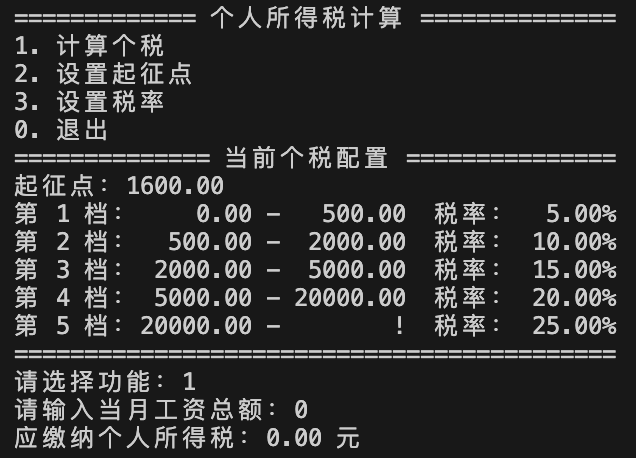
\includegraphics[width=0.5\textwidth]{image/TC1.png}
	\caption{测试用例TC1：收入为0，税额应为0}
	\label{fig:tc1}
\end{figure}

\subsection{测试用例二}

测试用例TC2：收入为1600，税额应为0

\begin{figure}[htbp]
    \centering
    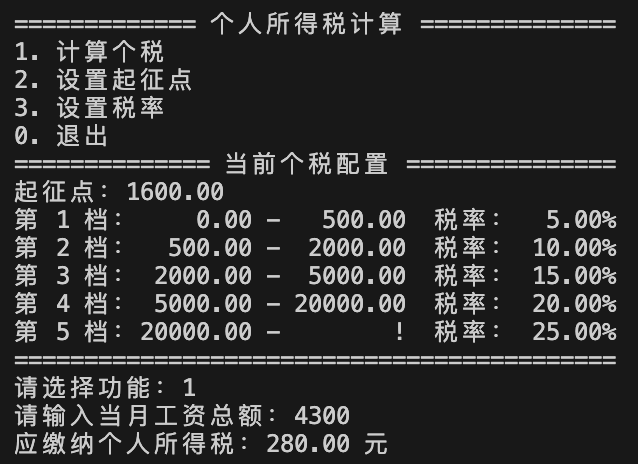
\includegraphics[width=0.5\textwidth]{image/TC2.png}
	\caption{测试用例TC2：收入为1600，税额应为0}
	\label{fig:tc2}
\end{figure}

\subsection{测试用例三}

测试用例TC3：收入为4300，税额应为280

\begin{figure}[htbp]
    \centering
    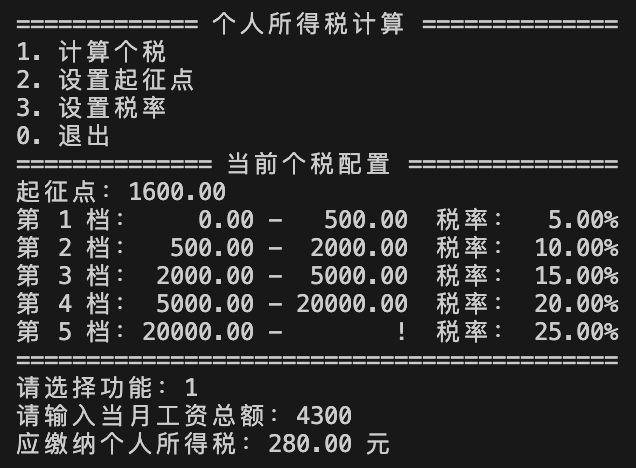
\includegraphics[width=0.5\textwidth]{image/TC3.png}
	\caption{测试用例TC3：收入为4300，税额应为280}
	\label{fig:tc3}
\end{figure}

\subsection{测试用例四}

测试用例TC4：收入为5000，税额应为385

\begin{figure}[htbp]
    \centering
    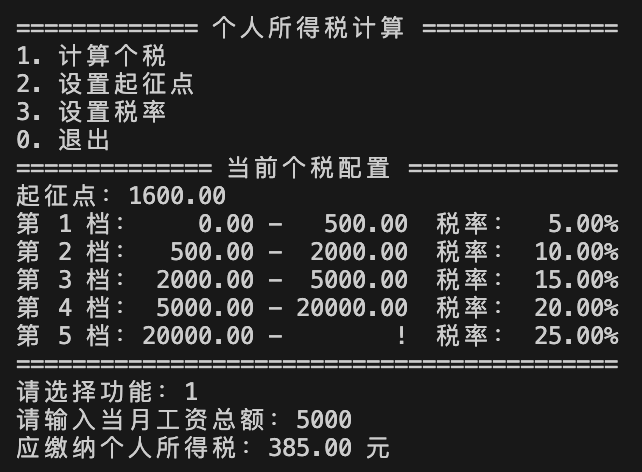
\includegraphics[width=0.5\textwidth]{image/TC4.png}
	\caption{测试用例TC4：收入为5000，税额应为385}
	\label{fig:tc4}
\end{figure}

\subsection{测试用例五}

测试用例TC5：收入为负数，抛出异常

\begin{figure}[htbp]
    \centering
    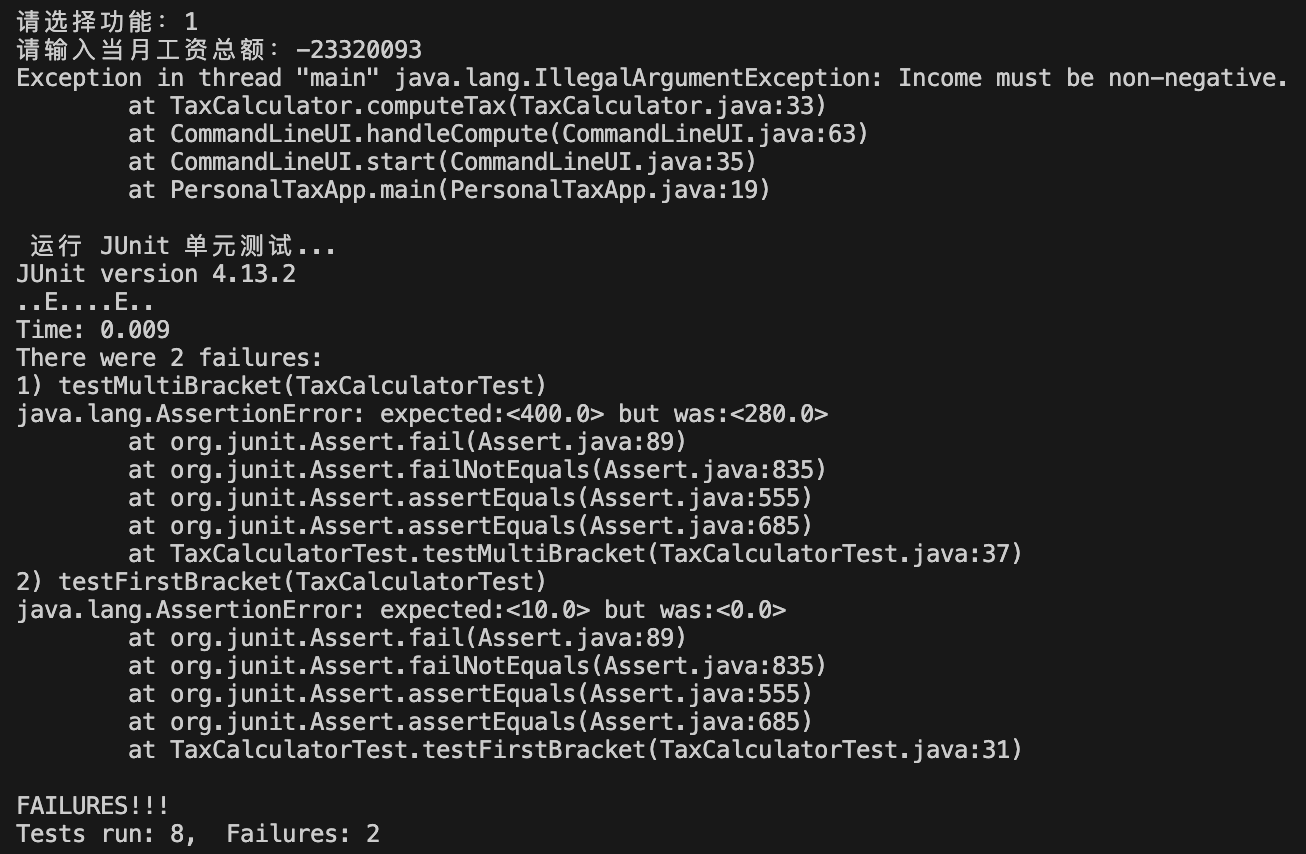
\includegraphics[width=0.8\textwidth]{image/TC5.png}
	\caption{测试用例TC5：收入为负数，抛出异常}
	\label{fig:tc5}
\end{figure}

\subsection{调整税额计算算法功能说明}

\subsection{调整起征点}

\begin{figure}[htbp]
    \centering
    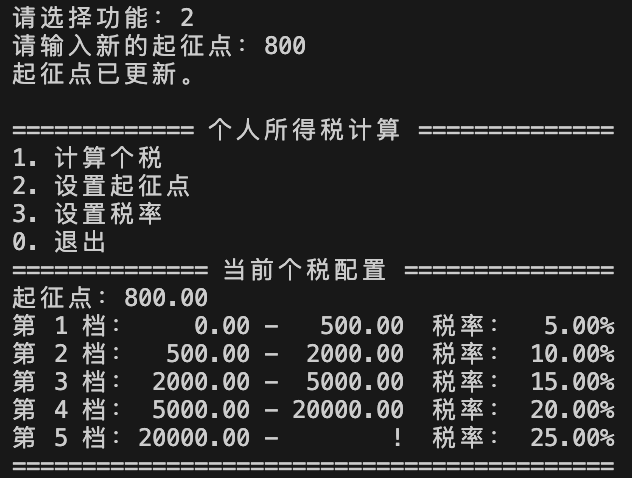
\includegraphics[width=0.5\textwidth]{image/fun1.png}
	\caption{调整起征点}
	\label{fig:fun1}
\end{figure}

\subsection{调整各级税额计算}

\begin{figure}[htbp]
    \centering
    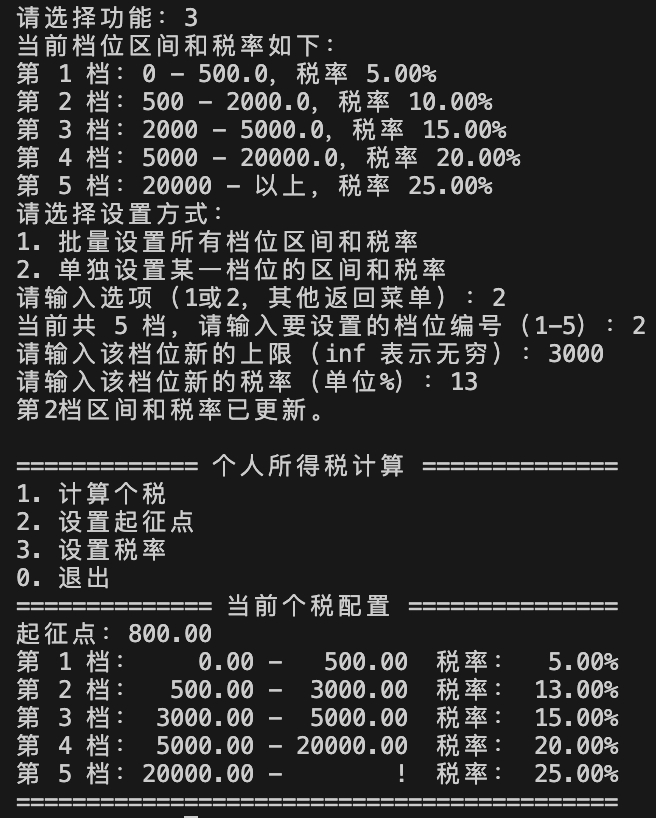
\includegraphics[width=0.5\textwidth]{image/fun2.png}
	\caption{调整各级税额计算}
	\label{fig:fun2}
\end{figure}

\subsection{配置设置异常检测}

\begin{figure}[htbp]
    \centering
    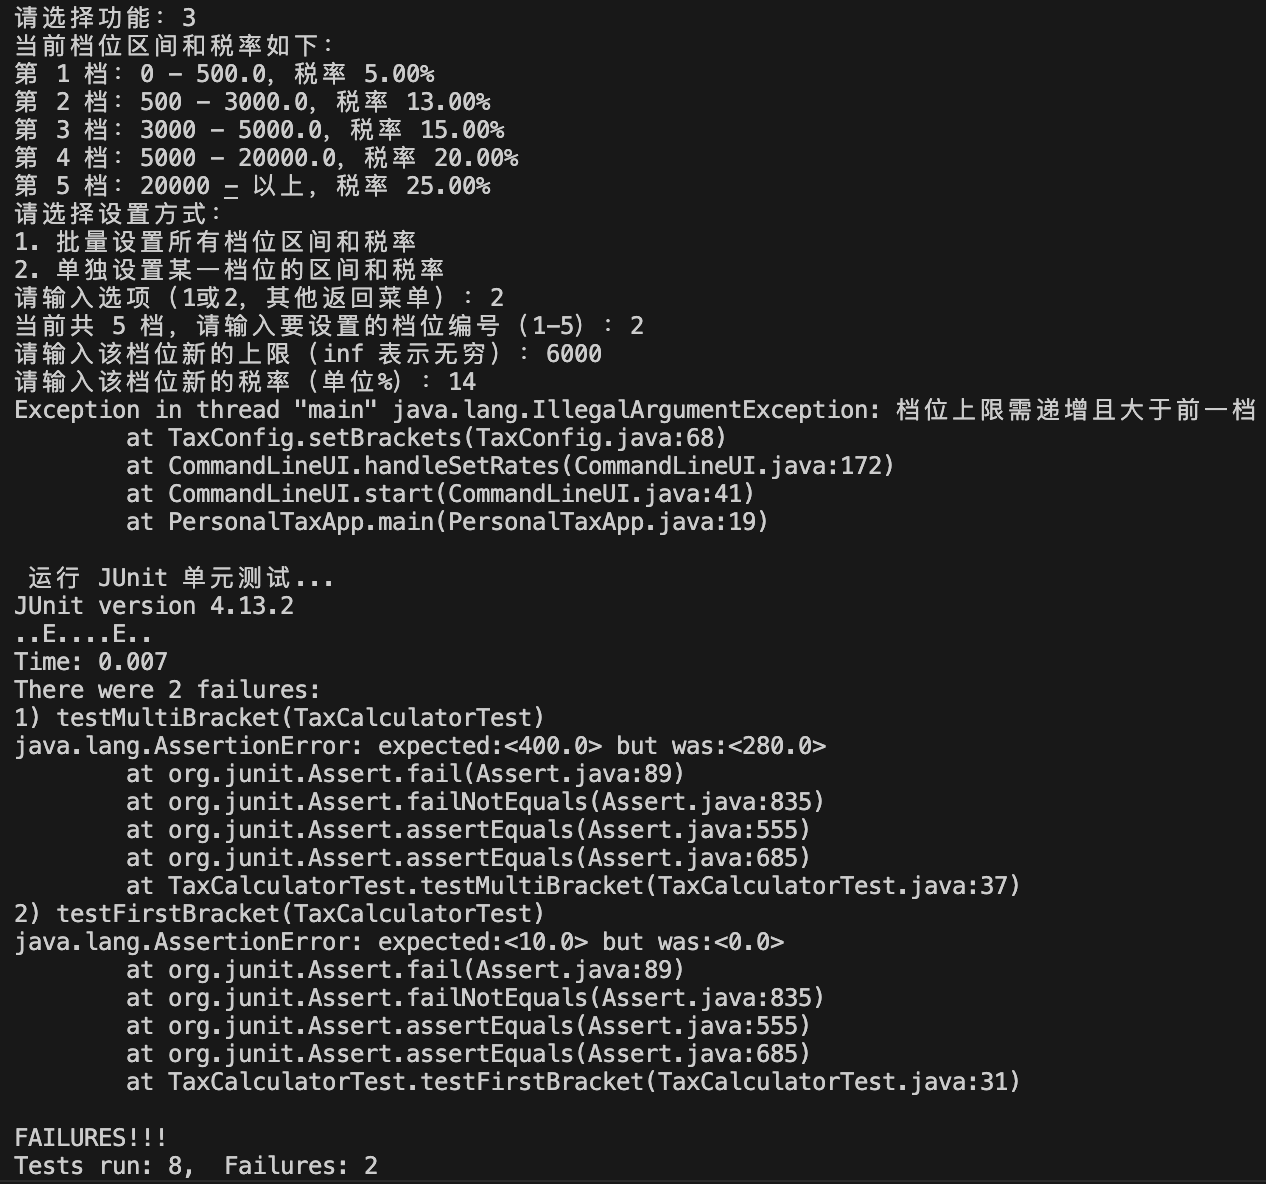
\includegraphics[width=0.8\textwidth]{image/fun3.png}
	\caption{配置设置异常检测}
	\label{fig:fun3}
\end{figure}

\section{代码}


核心算法代码展示如下，采用 Java 语言实现：

\definecolor{codebg}{RGB}{248,249,250}
\definecolor{codeframe}{RGB}{220,223,228}
\definecolor{codekw}{RGB}{25,85,145}
\definecolor{codecm}{RGB}{90,125,90}
\definecolor{codestr}{RGB}{136,44,136}
% Java代码风格
\lstdefinestyle{cleanjava}{
  language=Java,
  basicstyle=\ttfamily\small,
  keywordstyle=\bfseries\color{codekw},
  commentstyle=\itshape\color{codecm},
  stringstyle=\color{codestr},
  backgroundcolor=\color{codebg},
  frame=single,
  rulecolor=\color{codeframe},
  framesep=6pt,
  numbers=left,
  numberstyle=\scriptsize\color{gray},
  numbersep=8pt,
  breaklines=true,
  breakatwhitespace=false,
  showstringspaces=false,
  keepspaces=true,
  tabsize=4,
  columns=fullflexible
}

\subsection{TaxCalculator.java}
\lstinputlisting[style=cleanjava,caption={TaxCalculator.java},label={lst:tax-calculator}]{./code/TaxCalculator.java}

\subsection{TaxConfig.java}
\lstinputlisting[style=cleanjava,caption={TaxConfig.java},label={lst:tax-config}]{./code/TaxConfig.java}

\subsection{TaxBracket.java}
\lstinputlisting[style=cleanjava,caption={TaxBracket.java},label={lst:tax-bracket}]{./code/TaxBracket.java}

\subsection{CommandLineUI.java}
\lstinputlisting[style=cleanjava,caption={CommandLineUI.java},label={lst:cli-ui}]{./code/CommandLineUI.java}

\subsection{PersonalTaxApp.java}
\lstinputlisting[style=cleanjava,caption={PersonalTaxApp.java},label={lst:main-app}]{./code/PersonalTaxApp.java}
